\documentclass[a4paper]{jarticle}
% \documentclass[a5j]{jsarticle}


\usepackage{amsfonts,latexsym}
\usepackage{ulem}
\usepackage{fancybox}
\usepackage[dvipdfmx]{graphicx}
\usepackage[deluxe]{otf}
\usepackage[margin=20truemm]{geometry}

\usepackage{pifont}

\DeclareFontShape{JT1}{hmc}{b}{n}{<->ssub*hmc/bx/n}{}
\DeclareFontShape{JY1}{hmc}{b}{n}{<->ssub*hmc/bx/n}{}

% ==============================================
% page format
%  textwidth  = paperwidth(210mm) -oddsidemargin(13mm) -evensidemargin(13mm)
%  textheight = paperheight(297mm) -topmargin(20mm-header分) -bottommargin(18mm)
% ==============================================
  \setlength{\paperwidth}{210mm}
  \setlength{\textwidth}{\paperwidth}
  \addtolength{\textwidth}{-13mm} % oddside margin
  \addtolength{\textwidth}{-13mm} % evenside margin
  \setlength{\oddsidemargin}{-1in}
  \addtolength{\oddsidemargin}{13mm} %%%% ここで左右を調節
%
  \setlength{\paperheight}{297mm}
  \setlength{\textheight}{\paperheight}
  \addtolength{\textheight}{-10mm} % 文章領域の高さの調整
  \addtolength{\textheight}{-23truemm}  
  \setlength{\topmargin}{-17mm}    % ここで上下位置を調節
%
  \setlength{\headheight}{0in}
  \setlength{\headsep}{0in}
  \setlength{\columnsep}{10mm}

%   \pagestyle{plain}
  \pagestyle{empty}

% ========================================
% タイトルの書式設定(開始)
  \makeatletter
   \def\@maketitle{%
   \newpage\null
   \vskip 2em%
   \begin{center}%
   \let\footnote\thanks
     \vspace{-15mm}
     {\LARGE \@title \par}%
     \vskip 1.5em%
   \end{center}
   \begin{flushright}
     {\large
       \lineskip .5em%
       \begin{tabular}[t]{c}%
         \@author
       \end{tabular}\par}%
     \vskip 1em%
%      {\large \@date}%
   \end{flushright}%
   \par\vskip 1.5em}
   \vspace{10mm}
   \renewcommand{\section}{\@startsection{section}{1}{\z@}%
   {1.5\Cvs \@plus.5\Cvs \@minus.2\Cvs}%
   {.5\Cvs \@plus.3\Cvs}%\and
   {\reset@font\large\bfseries}}   %section見出しの文字サイズをlargeに変更
   
   % 参考文献の書式設定
   \renewenvironment{thebibliography}[1]
{\section*{\refname\@mkboth{\refname}{\refname}}%
  \list{\@biblabel{\@arabic\c@enumiv}}%
       {\settowidth\labelwidth{\@biblabel{#1}}%
        \leftmargin\labelwidth
        \advance\leftmargin\labelsep
%  \setlength\itemsep{-0.5zh}%←ここの数値を調整(行間のつまり具合)
 \setlength\baselineskip{12pt}%←ここの数値を調整(追加)(文字の大きさ)
        \@openbib@code
        \usecounter{enumiv}%
        \let\p@enumiv\@empty
        \renewcommand\theenumiv{\@arabic\c@enumiv}}%
  \sloppy
  \clubpenalty4000
  \@clubpenalty\clubpenalty
  \widowpenalty4000%
  \sfcode`\.\@m}
 {\def\@noitemerr
   {\@latex@warning{Empty `thebibliography' environment}}%
  \endlist}
  \makeatother
% タイトルの書式設定(終わり)
% ========================================


%ここから下を変更する
  \title{C2Cシェアサイクル実現に向けた人と自転車のマッチング最適化}
  \author{風折晃輝}
  \date{\today}


\fontsize{10.5mm}{0pt}

\begin{document}

\twocolumn[
 \begin{center}
  {\Large 第1回KP}\\
  \rule{\textwidth}{1mm}
 \end{center}
 \maketitle
  \thispagestyle{empty}
]


% 本文 =====================================

%\noindent

% section 1 ----
\section{はじめに}
\vspace{-3mm}
\par シェアサイクルとは,「相互利用可能な複数のサイクルポートが設置された,面的な都市交通に供されるシステム」と定義されており,自転車が設置されているサイクルポートを起点としてその自転車をシェアリングするシステムを指す.そのようなシェアサイクルを提供してる既存のサービスとして「LUUP」や「ドコモバイクシェア」等のサービスが挙げられる.これらのサービスではそれぞれのベンダーがサイクルポートを設置し,そのサイクルポートに自転車を準備することによってユーザーにサービスを提供する構造になっているため,自ずと人口が多くて需要の高い都市部や主要な駅周辺において集中的にサービスが提供されやすい形態となっている.一方で,比較的需要の低いとされている人口が少ない地方や駅から離れた地域ではシェアサイクリングサービスが提供されていないことが多く,そのような地域でも一定の需要は存在すると考えられる中で,シェアサイクリングサービスを利用したい人が利用できない状態になっている.
\par そこで,シェアサイクリングサービスが普及していない地域ではそのサービスを利用したい需要に対応できていない点を課題として挙げ,本研究ではその課題を解決するためのソリューションとして個人間でシェアリングできるシステムの構築を目指す.今回の発表においては,その部分要素となり得る人と自転車を最適にマッチングするためのアプローチについて述べる.

\vspace{-5mm}

% section 2 ----
\section{モデリングの導入}
\vspace{-3mm}
\par 自転車の個人間シェアリングシステムを実現するにあたって,利用した自転車を個人所有者のもとに返却しなければならない点がボトルネックの1つとして挙げられる.個人間のシェアリングであったとしても乗り捨てが可能であればよりモビリティーの自由度が向上することが期待される.そこで,できる限り乗り捨てを可能とするシステムを構築するため,シェアサイクルサービスのユーザーの目的地と自転車の本来あるべき場所(個人所有者の元)のデータを利用して人と自転車をマッチングする数理最適化を行い,モデリングする.

\vspace{-5mm}

% section 3 ----
\section{課題の整理と定義}
\vspace{-3mm}
\par モデルに落とし込むべき課題を整理する.最終目的としては,「乗り捨て可能な個人間シェアサイクルシステムを構築した際に,自転車とその所有者との位置関係(分散)を最小化する」こととする.その上で考慮するべき課題や制約は以下の通りになる.\\

\begin{tabular}{|c|p{5cm}|} \hline
 最小化指標 & 自転車の分散 \\ \hline
 マッチング要件 & 人(利用者)の目的地を予め取得できていることとし,自転車→所有者の方向性を考慮する. \\ \hline
 最適化対象期間 & 自転車の所有者が,少なくともいつまでに手元にないと困るかの期間を指定. \\ \hline
\end{tabular}

\vspace{-5mm}

% section 4 ----
\section{数理モデリング}
\vspace{-3mm}
\par 実験データとして,乗り捨てられた複数の自転車と,その自転車の所有者の座標(ホームポジション)をそれぞれランダムに生成する.また,所有者の手元に配置されている乗り捨てされていない自転車についてもランダムな座標を生成する.乗り捨てされている自転車の場合は自転車の現在地からホームポジションまで矢印で表現した分布図が図\ref{fig:乗り捨て可能な個人間シェアリングの自転車分布図}のようになる.なお,赤い星はユーザーの現在地を示す.当日までになんらかの結果が出れば結果について述べる.

\begin{figure}[htbp]  % [H]はこの場所に置くって意味, 無いと適当な空きスペースに図が自動で飛ばされる
  \centering
    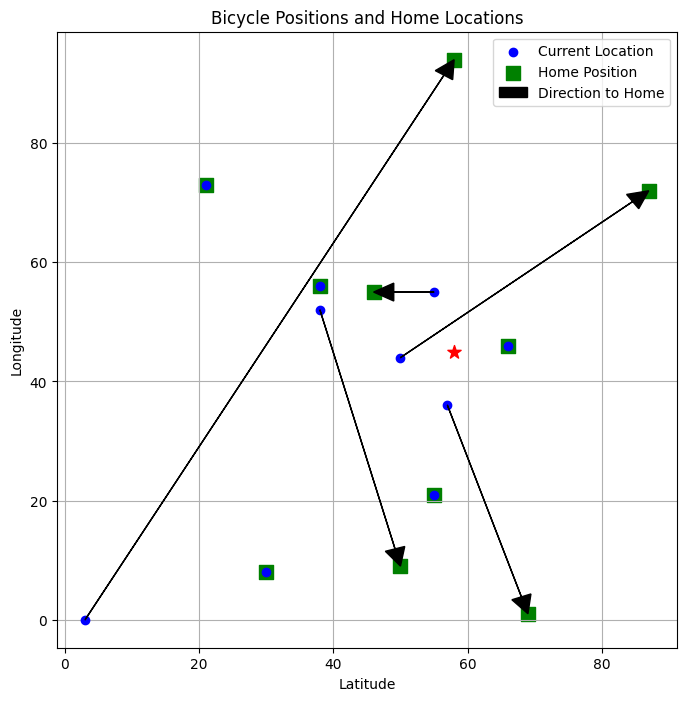
\includegraphics[scale=0.38]{figures/bikePositionsAndHomeLocations.png}
  \caption{乗り捨て可能な個人間シェアリングの自転車分布図}
  \label{fig:乗り捨て可能な個人間シェアリングの自転車分布図}
\end{figure}

\vspace{-8mm}

% section 5 ----
\section{まとめと今後の方針}
\vspace{-3mm}
個人間シェアリングシステムに実装するにあたって,より制約条件をスケールしていく必要がある.例えば,「分散を最小化する」かつ「システムの収益を最大化する」という最小化指標と最大化指標の複数指標で議論しなければならない.ただ,分散を最小化することを最優先として考え,より最適なモデルを構築することを目指す.

\vspace{-3mm}

% \bibliographystyle{junsrt}
% \bibliography{sannkou.bib}
% ==============================================
% 原稿はここまで
% ==============================================
\end{document}
